\documentclass{sigchi}

\toappear{\scriptsize Permission to make digital or hard copies of all or part of this work for personal or classroom use is granted without fee provided that copies are not made or distributed for profit or commercial advantage and that copies bear this notice and the full citation on the first page. Copyrights for components of this work owned by others than ACM must be honored. Abstracting with credit is permitted. To copy otherwise, or republish, to post on servers or to redistribute to lists, requires prior specific permission and/or a fee. Request permissions from permissions@acm.org. \\
	{\emph{L@S 2016}}, April 25--26, 2016, Edinburgh, UK. \\
	Copyright \copyright~2016 ACM 978-1-4503-3726-7/16/04\ ...\$15.00. \\
	DOI: \url{http://dx.doi.org/10.1145/2876034.2876038}}
\clubpenalty=10000 
\widowpenalty = 10000

% Load basic packages
\usepackage{balance}  % to better equalize the last page
\usepackage{graphics} % for EPS, load graphicx instead 
\usepackage{mathptmx}
\usepackage[pdftex]{hyperref}
\usepackage{color}
\usepackage{booktabs}
\usepackage{textcomp}
\usepackage{microtype} % Improved Tracking and Kerning
\usepackage{ccicons}  % Cite your images correctly!
\usepackage{multicol}
\usepackage{balance}
\usepackage{color} 
\newcommand{\hl}[1]{\colorbox{yellow}{#1}}
\usepackage{xspace}
\usepackage{algorithm} 
\usepackage[noend]{algpseudocode}
\usepackage{subcaption}
\usepackage{booktabs}
\def\algname{SPRING\xspace}
\DeclareMathOperator*{\argmin}{argmin}
\DeclareMathOperator*{\argmax}{argmax}
\usepackage{wrapfig, subcaption}

\usepackage{adjustbox}
\usepackage{tikz}
\usetikzlibrary{shapes,arrows,positioning} 
\tikzset{
	%Define standard arrow tip
	>=stealth',
	% Define arrow style
	pil/.style={
		<-,
		shorten <=0pt,
		shorten >=0pt,}
}

\floatname{algorithm}{Procedure}
\renewcommand{\algorithmicrequire}{\textbf{Input:}}
\renewcommand{\algorithmicensure}{\textbf{Output:}}


\usepackage{tikz}
\usetikzlibrary{decorations.pathreplacing,calc}
\newcommand{\tikzmark}[1]{\tikz[overlay,remember picture] \node (#1) {};}
\newcommand*{\AddNote}[4]{%
	\begin{tikzpicture}[overlay, remember picture]
	\draw [decoration={brace,amplitude=0.2em},decorate, thick, darkgray]
	($(#3)!(#1.north)!($(#3)-(0,1)$)$) --  
	($(#3)!(#2.south)!($(#3)-(0,1)$)$)
	node [align=left, text width=2.5cm, pos=0.5, anchor=west] {#4};
	\end{tikzpicture}
}%


% Paper metadata (use plain text, for PDF inclusion and later
% re-using, if desired).  Use \emtpyauthor when submitting for review
% so you remain anonymous.
\def\plaintitle{A Data-Driven Approach for Inferring Student Proficiency from Game Activity Logs  }
\def\plainauthor{Mohammad H. Falakmasir, Jos\'{e} P. Gonz\'{a}lez-Brenes, Geoffrey J. Gordon, Kristen E. DiCerbo}
\def\emptyauthor{}
\def\plainkeywords{Authors' choice; of terms; separated; by
	semicolons; include commas, within terms only; required.}
\def\plaingeneralterms{Documentation, Standardization}


% llt: Define a global style for URLs, rather that the default one
\makeatletter
\def\url@leostyle{%
	\@ifundefined{selectfont}{
		\def\UrlFont{\sf}
	}{
	\def\UrlFont{\small\bf\ttfamily}
}}
\makeatother
\urlstyle{leo}

% To make various LaTeX processors do the right thing with page size.
\def\pprw{8.5in}
\def\pprh{11in}
\special{papersize=\pprw,\pprh}
\setlength{\paperwidth}{\pprw}
\setlength{\paperheight}{\pprh}
\setlength{\pdfpagewidth}{\pprw}
\setlength{\pdfpageheight}{\pprh}

% Make sure hyperref comes last of your loaded packages, to give it a
% fighting chance of not being over-written, since its job is to
% redefine many LaTeX commands.
\definecolor{linkColor}{RGB}{6,125,233}
\hypersetup{%
	pdftitle={\plaintitle},
	% Use \plainauthor for final version.
	%  pdfauthor={\plainauthor},
	pdfauthor={\emptyauthor},
	pdfkeywords={\plainkeywords},
	bookmarksnumbered,
	pdfstartview={FitH},
	colorlinks,
	citecolor=black,
	filecolor=black,
	linkcolor=black,
	urlcolor=linkColor,
	breaklinks=true,
}

% create a shortcut to typeset  headings
% \newcommand\tabhead[1]{\small\textbf{#1}}

% End of preamble. Here it comes the document.
\begin{document}
	
	
	\title{\plaintitle}
	
	\numberofauthors{4}
	\author
	{%
		\alignauthor{\mbox{\hspace{-1.85em}Mohammad H. Falakmasir$^{\star, \#} $\;\;\; Jos\'{e} P. Gonz\'{a}lez-Brenes$^\star$ \;\;\; Geoffrey J. Gordon$^\S$ \;\;\; Kristen E. DiCerbo$^\star$}\\
			\affaddr{$^\star$School Research}\\
			\affaddr{Pearson}\\
			\email{\{jose.gonzalez-brenes, kristen.dicerbo\}@pearson.com }\\
		}
		\alignauthor{\vphantom{Mohamamad Jose}
			\affaddr{$^\#$Intelligent Systems Program} \\
			\affaddr{University of Pittsburgh}\\
			\email{falakmasir@pitt.edu}\\
		}
		\alignauthor{\vphantom{Mohamamad Jose}
			\affaddr{$^\S$Machine Learning}\\
			\affaddr{Carnegie Mellon University} 
			\email{ggordon@cs.cmu.edu}\\
		}
	}
	
	
	\maketitle
	
	\begin{abstract}
		Student assessments are important because they allow collecting evidence about learning. 
		However,  time spent in  evaluating students may have been otherwise  used for instructional activities.
		Computer-based learning platforms provide the opportunity for unobtrusively gathering students' digital learning footprints.
		This data can be used to track learning progress and make inference about student competencies.
		We present a novel data analysis pipeline, {Student Proficiency Inferrer from Game data} (\algname), that allows modeling  game playing behavior in educational games.
		Unlike prior work, \algname is a fully data-driven method that does not require costly domain knowledge engineering.
		Moreover, it produces a simple interpretable model that not only fits the data, but also predics learning outcomes.
		We validate our framework using data collected from students playing 11 educational mini-games.
		Our results suggest that \algname can predict math assessments accurately on withheld test data (Correlation=0.55, Spearman $\rho$=0.51).
	\end{abstract}
	
	%	\category{K.3.1}{Computer Uses in Education.}
	%	{}
	\keywords{Educational Games, Student Modeling, Stealth Assessment}
	
	\section{Introduction}
	Educational assessments are important because they collect evidence about  whether instructional goals are achieved or not.
	Unfortunately, the process of  administering assessments is usually disconnected from the instructional environment, and  it is often  disruptive to the learning experience. 
	In many developed countries, students now find themselves spending increasing amounts of time preparing for and taking tests instead of learning~\cite{hofman2015re}.
	For example, a  survey of the current state of testing in America revealed that students are taking an average of 113 standardized tests between pre-K and highschool~\cite{lazarin2014testing}. 
	For these reasons, it is not surprising that both politicians and the general population have been weighing in on the question of whether students are being tested too much~\cite{lazarin2014testing}.
	
	Learning and succeeding is not easily measured by solving constrained tasks and answering verbal or multiple-choice questions.
	Advancements in educational  measurements allow us to diagnose student competencies more accurately and effectively at various levels during the course of learning.
	According to Evidence Centered Design (ECD)~\cite{mislevy2012design}, the goal of assessment is to characterize the evidence regarding claims one wants to make about the competencies of individuals or groups of students.
	The assessment process involves identifying, organizing, or creating activities for students so that we may observe that evidence.
	An alternative to traditional summative assessment (e.g, exams) is to use data collected from computer based learning environments.
	This data can be used for invisible (or stealth) assessment~\cite{shute2013stealth}.
	One of the advantages of invisible assessment is to blur the distinction between assessment and learning.
	
	Analyzing log data collected from students playing educational games is a  promising way to perform invisible assessment.
	Studying the sequence of actions in an educational game provides incremental evidence about mastery of specific skills and allows us to infer what students know at any point in time.
	Prior studies have also reported that invisible assessment may reduce test anxiety, while not sacrificing validity and reliability of the results~\cite{shute2008you}.
	Unfortunately, engineering a system that interprets log data is costly and time-consuming.
	For example, Shute et al.~\cite{shute2013stealth, shute2009melding} relied extensively on domain expertise to define a \textit{Competency Model} in form of a Bayesian Network to describe the set of knowledge and skills involved in the learning environment.
	They also conducted feature engineering on the performance data to build an \textit{Evidence Model} that expresses how student interactions with the system constitute evidence about competency model variables.
	
	
	In this paper, we propose \textit{Student PRoficiency INferrer from Game data} (SPRING), a novel data analysis pipeline that models game playing behavior.
	Our motivation is that invisible assessment from game data may become more accurate and cheaper to implement if the domain knowledge engineering could be automated by a data-driven process.
	Our experiments suggest that \algname is able to capture student differences and provide features that can be used to predict student proficiency.
	The rest of this paper is organized as follows:
	\S~\ref{sec:game_data}   describes the specific challenges that makes game data  difficult to analyze;
	\S~\ref{sec:spring} details the SPRING algorithm;
	\S~\ref{sec:experiments} evaluates the SPRING algorithm with student data;
	\S~\ref{sec:priorwork} relates to prior work;
	\S~\ref{sec:conclusion} provides concluding remarks.
	
	
	\section{Background}
	\label{sec:game_data}
	Game data is often logged  in a format that we call a \textit{slot and filler}.
	In Table~\ref{tbl:log_example}, we show a simplified example of a real educational game log that uses slot and filler structure.
	Typically each action or event has a set of slots (properties).
	Each slot may accept zero to multiple fillers. 
	Each filler represents a property value of the slot.
	For example, a \texttt{Move Object} event  that represents the learner moving an object in the screen may have a $x$ and $y$ coordinates as slots and the target position in two-dimensional space ($361, 82$) are the fillers.
	\newline
	
	\begin{table}[tbh]
		\begin{tabular}{@{}llll@{}}
			\toprule
			\textbf{Id}             & \textbf{User Id} & \textbf{Event Name} & \textbf{Event Data}        \\ \midrule
			1                       & ABC              & Game Start          & \{ \}                        \\
			2                       & ABC              & Move Object         & \{X:363,Y:82\} \\
			3                       & ABC              & Move Object         & \{X:361,Y:54\} \\
			4                       & ABC              & Open Toolbox        & \{\}        \\
			5                       & ABC              & Activate Tool        & \{tool:gluumi\}        \\
			6                       & ABC              & Use Gluumi        & \{sizeGluedTo:8,sizeNew:9\} \\        
			\multicolumn{1}{c}{...} &                  &                     &                            \\ \bottomrule
		\end{tabular}
		\caption{An example fragment of a log from an educational game. \label{tbl:log_example}}
	\end{table}
	
	Analyzing slot and filler data is difficult.
	Some general-purpose predictive models (like logistic regression or decision trees)  that are used in off-the-shelf data mining packages, such as Weka \cite{hall2009weka}, often use a vector representation of features as input. 
	A vector representation requires mapping of observations onto a fixed number of features.
	It is not obvious how to best map the sequence of events (in slot-and-filler format)  into feature vectors.
	Feature vectors need to be of a predetermined dimension, and a game log may have a variable number of slots.
	
	Machine learning algorithms that are able to work with data that is not represented as feature vectors include kernel methods and graphical models.
	To the extent of our knowledge, there are no kernels designed specifically for slot and filler structures.
	Popular general-purpose graphical models, such as Markov Models and Hidden Markov Models (HMM), allow sequence data with a variable number of events.
	However, these models require that each time step is represented with observations with the same number of dimensions.
	This is not possible when the number of fillers can vary for different slots.
	For example, in Table~\ref{tbl:log_example}, the \texttt{Move Object} requires fillers with 2 dimensions, while the \texttt{Game Start} has no fillers.
	On the other had,  \textit{ad hoc} graphical models have  been proposed for mining specific games.
	However, these graphical models were tailored by subject matter experts, and do not generalize across different games \cite{rowe2010integrating}.
	
	\algname models slot and filler data for educational games when domain knowledge is too expensive or cumbersome to collect.
	To learn a \algname model, we need (i) logs  from students playing educational games, (ii) and  their results in  traditional assessments.
	\algname transforms the slot and filler data to sequences that can be modeled with Hidden Markov Models.
	It then extracts features from the sequences, and uses them in a regression model to predict the score of the traditional assessment.
	After this, \algname is able to predict assessment performance of students by just observing their game activity as described by their slot and filler log.
	
	\section{SPRING Algorithm}
	\label{sec:spring}
	
	
	\algname is designed in a way that can capture sequential decision making process of students in a way that is representative of their mastery with minimum reliance on expert knowledge. 
	Our data analysis pipeline receives raw data of student interactions in slot and filler format along with their post-test results.
	Once a \algname is learned, it can be used to predict  post-test scores from game playing data.

	\begin{algorithm}[ht]
		\begin{algorithmic}[1]
			\Require: A log file $\mathbf{L_{g,s,t}}$ of slot and filler structure for each game $g$ and student $s$ (indexed by time $t$),  results from a student assessment $y_s$, number of performance clusters $K$, number of latent states $H$.
			\For {each  game $g$}  \tikzmark{disctop}
			\State $\mathbf{D_{g,s,t}} \leftarrow$  Discretize\_Fillers($\mathbf{L_{g,s,t}}$) 
			\State  $\langle s, c \rangle \leftarrow$  Cluster\_Students($y_s, K$)  \tikzmark{discbot}
			\For {each student performance group $c$} \tikzmark{seqmodtop} \tikzmark{right}
			\State  $\mathbf{D_c} \leftarrow \mathbf{D_{g,s,t}}$ where $s \in \langle s, c \rangle$  
			\State$\theta_{g, c} \leftarrow$  Learn\_HMM($\mathbf{D_c}, H$) 
			\EndFor\tikzmark{seqmodbot}
			\EndFor 
			\For{each sequence $d$ in $\mathbf{D_{g,s}}$}  \tikzmark{regtop}
			\State  $\phi_{g,s} \leftarrow$  Extract\_Features($d,\theta_{g,c}$)  
			\EndFor
			\State Learn a model that predicts $y_s$  from $\phi_{g,s}$ 
			\tikzmark{regbot}
		\end{algorithmic}
		\AddNote{disctop}{discbot}{right}{\scriptsize{Discretization}}
		\AddNote{seqmodtop}{seqmodbot}{right}{\scriptsize{Sequence Model}}
		\AddNote{regtop}{regbot}{right}{\scriptsize{Feature \\ Vector Model}}
		\caption{The SPRING algorithm\label{alg:spring}}
	\end{algorithm}
	
	Procedure~\ref{alg:spring} describes the three main steps of our pipeline: discretization,  sequence modeling, and feature vector modeling.
	The discretization step transforms slot and filler observations into multinomial indicators that are used as evidence for learning.
	The sequence modeling step learns a representation from data in the form of a Hidden Markov Model for high- and low-performing students.
	The feature vector modeling step, uses the likelihood of student sequences in each game level as feature to predict the post-test results.
	We now explain the different steps in detail.

	
	\subsection{Discretization}
	We now describe how we discretize
	the slot and fillers  (\S~\ref{sec:filler_disc}) 
	and the student performance (\S~\ref{sec:student_disc}).
	
	\subsubsection{Slot-Filler Discretization}
	\label{sec:filler_disc}
	
	\begin{algorithm}[ht]
		\begin{algorithmic}[1]
			\Require: $L_{g,s,t}$, sequence of slot-and-filler observations in game level $g$
			\Procedure{Discretize\_Fillers}{$\mathbf{L_{g,s,t}}$}
			\State {$\mathbf{Z} \leftarrow$  enumerate\_slots($\mathbf{L_{g,s,t}}$)}
			\For{each slot $z$}
				\State{$\mathbf{F_{z} } \leftarrow$  get\_fillers($\mathbf{L_{g,s,t}}$)}
				\State{ $\langle \mathbf{F_{z}}$ , clustersIDs   $\rangle \leftarrow$ Cluster($\mathbf{F_{z}}$) } 
				\State{model  $\leftarrow$ learn\_classifier($\mathbf{F_{z}}$, clustersIDs) }
			\EndFor

			\State
			\For{each student $s'$}	
				\For{each time step $t'$}
					\If {$z$ == slot($L_{g,s',t'}$)}
						\State { $\hat f \leftarrow$  model.predict(filler($ L_{g,s',t'} $)) }
						\State {$d  \leftarrow $ \text{concat}(z, $\hat f$) }
						\State{$\mathbf{D_{g,s',t'}} \leftarrow  d$} 
				\EndIf
			\EndFor
			\EndFor
			\State \Return{ $\mathbf{D}_{g,s,t}$ }
			\EndProcedure
			
		\end{algorithmic}
		\caption{The Discretization Step of \algname \label{alg:discretize}}
	\end{algorithm}
	

	Procedure~\ref{alg:discretize} describes the method we use to discretize fillers for each game.
	The input is time-ordered student interactions in slot-and-filler format for a single slot $z$ and a game $g$.
	The purpose is to transform the slot and filler observations into  discrete (multinomial) observations appropriate for sequence modeling.
	For example, consider the \texttt{Move Object} slot from Table~\ref{tbl:log_example}.
	We wish to transform the different possible fillers into discrete units.
	Figure~\ref{fig:screenshot} shows a screenshot of a minigame that generates  \texttt{Move Object} slots.
	The purpose of this game is for learners to move ice cubes from the mountain top onto the two designated areas to prevent the Yeti from crossing the wall.
	Figure~\ref{fig:clustering} shows a scatterplot of the $x$ and $y$ fillers aggregating across 77 students.
	
	\begin{figure}[ht]
		\centering
		\begin{subfigure}[t]{.5\textwidth}
			\centering
			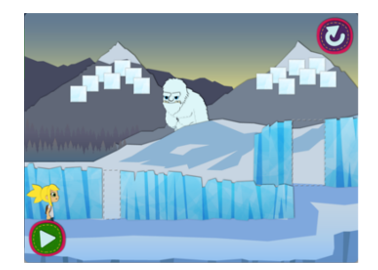
\includegraphics[width=0.9\columnwidth]{figures/glacier_screenshot.png}
			\caption{Screenshot of game level 2, \textit {None Shall Pass!} \label{fig:screenshot}}
		\end{subfigure}
		\begin{subfigure}[t]{.5\textwidth}
			\centering
			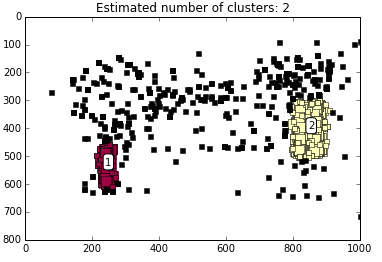
\includegraphics[width=0.9\columnwidth]{figures/glacier_positions.png}
			\caption{Clusters found using DBSCAN method. We transform each movement action into corresponding cluster id during the discretization step. \label{fig:clustering}}
		\end{subfigure}
		\caption{Analysis of the  \texttt{Move Object} slots and fillers from the \textit{None Shall Pass!} mini game\label{fig:figurecluster}}
	\end{figure}
	
	In order to transform the slot and filler observations into discrete events, we use an unsupervised clustering algorithm for the fillers of each slot.
	For example, in Figure~\ref{fig:clustering}, we have three clusters,  cluster one and two (red and yellow respectively) that represent frequent movements, and cluster zero (black) that represents ``outlier'' movements.
	We speculate that the outlier group is a result of either technical glitches in the gaming environment or student misconceptions.
	To build discrete events we use the  concatenation of slot and cluster labels as a  observations in the sequence modeling phase.
	For example, instead of modeling from an infinite  domain like ``\texttt{Move Object $\langle x:363, y:83 \rangle$}",
	we use a number of discrete observations like ``\texttt{Move Object Cluster 1}".
	
	The specific clustering algorithm we used  in our experiments is called DBSCAN~\cite{ester1996density}.
	In  preliminary experiments we tried other unsupervised methods, but  we found DBSCAN easier to use because it can find arbitrarily shaped clusters and does not require one to specify the number of clusters in advance.
	The time complexity of DBSCAN is $O(n \log n)$ (n = the number of data points) and there are recent parallelized implementations that are scalable \cite{dai2012efficient, patwary2012new}.
	
	Clustering algorithms like DBSCAN often can only discretize observations in the training dataset, and would not generalize to unseen fillers.
	To work around this limitation, we trained a classifier for transforming any filler into a cluster label. 
	In particular, we used a K-Nearest Neighbor (K-NN, n=5) classifier because, similar to DBSCAN, it uses a Euclidean distance function as a similarity metric.
	The classifier is trained to identify a cluster label using the fillers as predictors.
	The K-NN classifier might not be the best choice for fillers in the outlier cluster. 
	However, our preliminary experiments using cross-validation showed that it has enough discriminative power to distinguish the outlier fillers from other clusters.
	\newline
	
	\subsubsection{Student Performance Clustering}
	\label{sec:student_disc}

	While learning an \algname model, we group students according to their performance.
	A simple way to do this is by using the median of students' post-test scores to divide students into groups.  
	For example, by placing the students who received a post-test score below or equal to the median in the low-performing group and the students who received a post-test score higher than the median in the high-performing group.

	More sophisticated alternatives  grouping students would involve using a clustering algorithm, and tuning the number of groups.
	However, due to the small number of students in our dataset, particularly in the later game levels, we only used two clusters. 
	We hypothesize that students in difference performance groups play the game differently. 
	Our sequence modeling phase should be able to capture these differences by learning the interaction patterns of each group in different game levels.
	
	\subsection{Sequence Modeling}
	Once we have transformed the slot-and-filler structure into sequences of discrete observations, we can start looking for sequential patterns among different performance groups in each game level.
	Hidden Markov Models are a popular statistical tool for analyzing sequential patterns.
	We can model the sequence of student actions  as observations,
	and  infer a set of unobserved (latent) states.
	In this context the states describe the process that generated the observations, along with statistical patterns that can describe and distinguish those states.
	Learning the ``best" value for number of states ($H$) is a difficult problem in practice. 
	There has been considerable prior work on this problem that used penalized likelihoods \cite{rabiner1989hmm}, Monte-Carlo cross-validation \cite{smyth1996clustering}, and mixture of HMMs \cite{smyth1997clustering}.
	We used the Hierarchical Dirichlet Process HMM (HDP-HMM) \cite{fox2008hdp}, which allows state spaces of unknown size to be learned from data. 
	HDP-HMM defines a \textit{hierarchical Dirichlet process} prior on transition matrices over countably infinite state spaces and is able to make a principled choice of how many states it needs based on the complexity of its training data. 
	For details on training methods please refer to \cite{fox2008hdp}.
	
	In summary, for each game we discretize the slot and fillers to build sequences.  Then, we use the sequences to learn two HDP-HMMs for each game: one for high-performing students and one for low-performing students. 
	The two models can be considered as a stochastic representation of the sequence of actions and we can use them to infer the likelihood of any arbitrary sequence as a feature for the regression step. 
	
	\subsection{Feature Vector Modeling}

	Given a sequence of student data, we can determine how likely it is for the student to be in the high-performing group or in the low-performing group.
	We calculate this likelihood by estimating the Forward-Backward probabilities  on each student sequence of actions  based on the two HMMs models.
	Then, for each student $s$ in each game level $g$, we calculate the difference ($d_{s,g}$)  between the log-likelihood of observing the sequence of actions given the two models. 
	Since we are learning different HMMs for each game levels,
	we use a hyperbolic tangent function in order to convert the difference to a value between -1 and 1: 
	
	\begin{equation}
	d_{s,g} = tanh[ K * (\theta_{g, \text{high}} - \theta_{g, \text{low}})]
	\end{equation}
	
	This step simply scales and shifts the difference between  log-likelihoods in a way that if one HMM fits the
	data much better than the other, the value of $d_{s,g}$ is closer to one of the boundaries and when there is no clear difference the value would be close to zero. 
	The parameter K represents the scaling factor.
	Larger values for K result in output distribution that are closer to +1 and -1 in case of clear difference.
	We experimented with different K values across game levels and picked K=100.


	In the next step, we use the transformed log-likelihood differences in each game level as features of a linear regression model that predicts the post-test scores:

	\begin{equation}
	\hat {y_s}(\beta) =   \sum_g \beta_g \cdot d_{s,g}  + \beta_0
	\end{equation}
	
	Here, $\beta_0$ is an intercept for the  model.  
	We optimized the parameters of the model using a 5-fold cross validation on our development set.
	We experimented with different regularization methods, but only report LASSO~\cite{tibshirani1996regression} as it worked best in our preliminary comparisons:

	\begin{equation}
	\beta^* = \argmin_\beta || y_s - \hat{y_s}(\beta)  ||_2 + \lambda \cdot || \beta ||_1
	\end{equation}
	
	\section{Empirical Evaluation}
	\label{sec:experiments}
	
	
	We use data collected from an educational game called  \textit {Alice in AreaLand}.
	This game was developed for research purposes as a part of Pearson Insight Learning System\footnote{\url{http://researchnetwork.pearson.com/learning-science/insight-learning-system}}. 
	It focuses on teaching and assessing geometric measurement, specifically the understanding of area, among 6\textsuperscript{th} grade students. 
	The game targets three main stages in the development of area: 1) area unit iteration, 2) use of unit squares to measure area, and 3) use of composites to measure area. 
	The current version has 12 game levels. 
	A simple student scenario involves covering a 2D area with smaller unit squares placed end-to-end in non-overlapping fashion, combining the single squares into rows or columns, and then determining the number of rows or columns needed. 
	Figure~\ref{fig:figurekracken} shows a screenshot of one game level.
	
	\begin{figure}
		\centering
		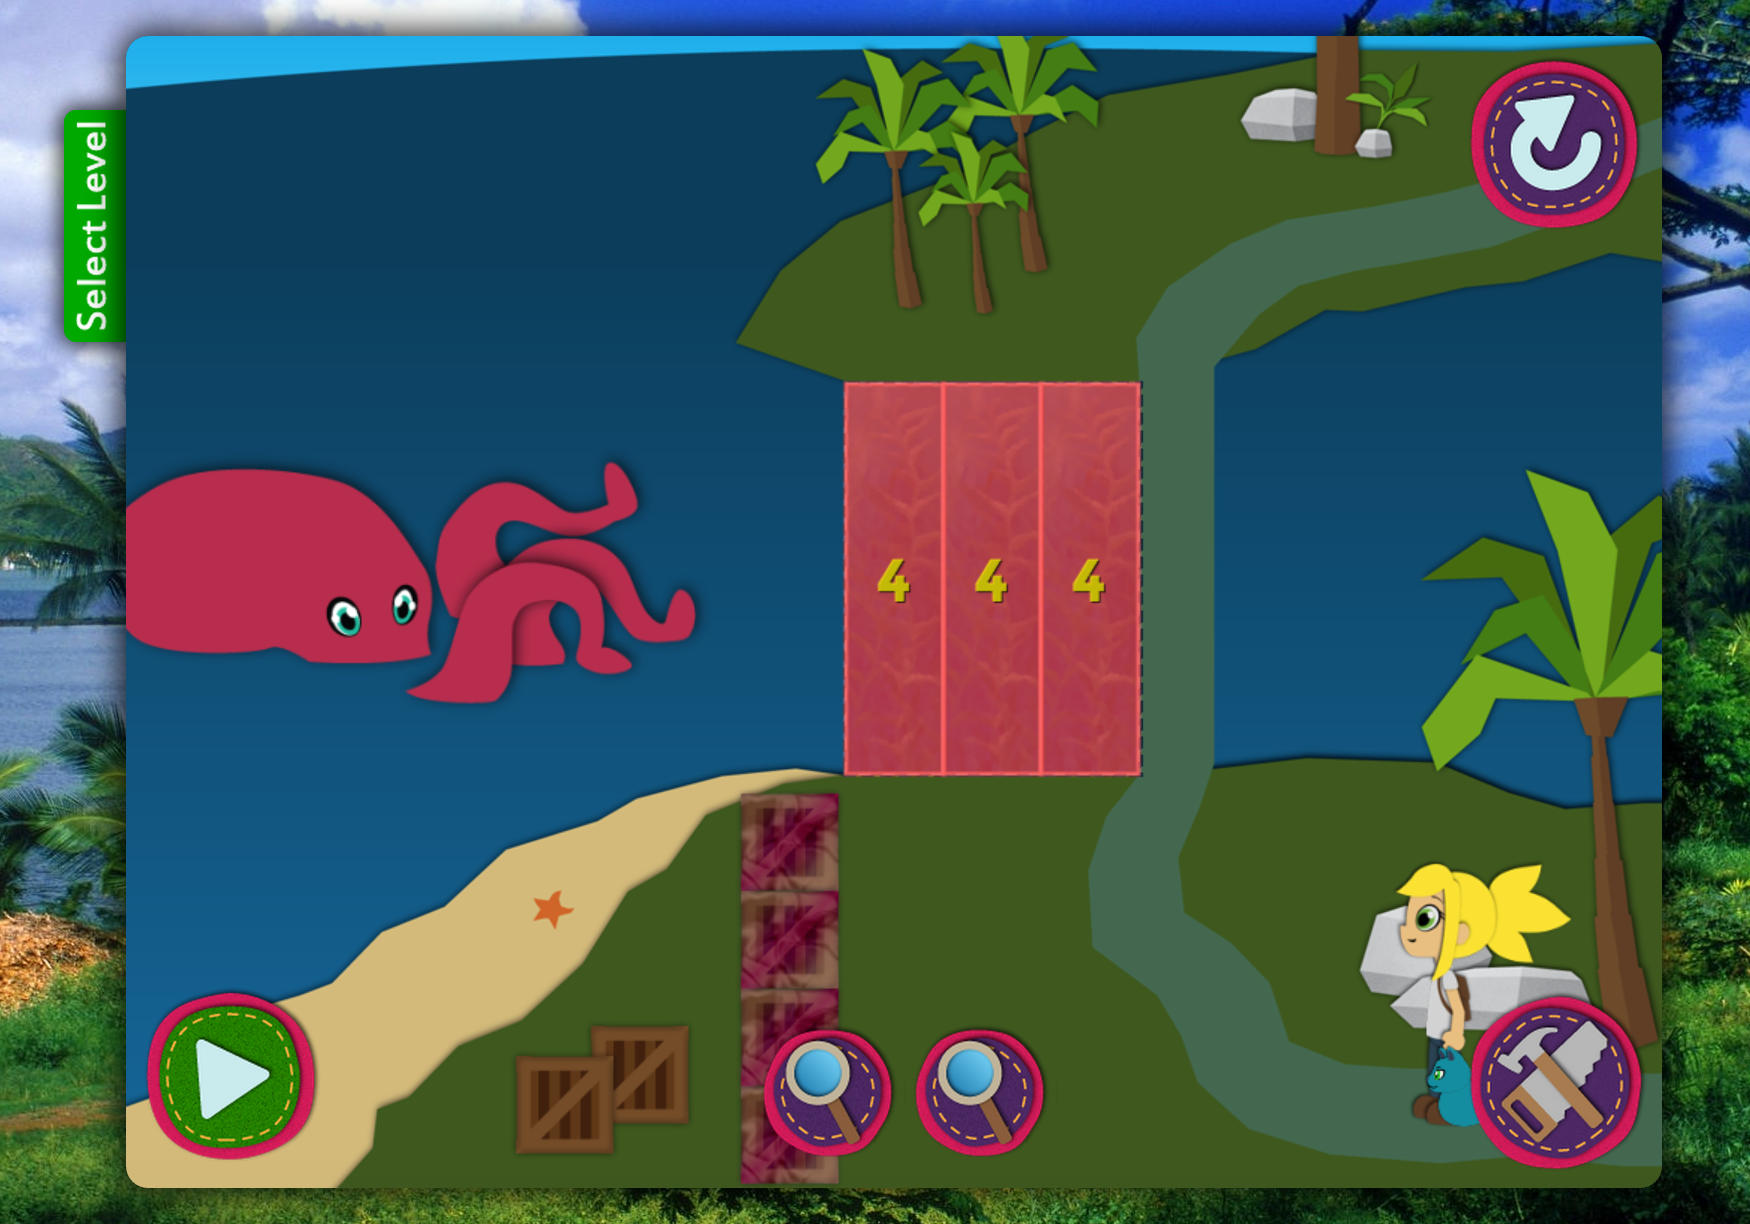
\includegraphics[width=0.9\columnwidth]{figures/kracken}
		\caption{A screenshot of hint provided in game level 11, ``You Kraken Me Up!", in Alice in AreaLand. Students should combine four squares into a column and create three copies of the column to cover the designated area and prevent the octopus from attacking Alice while she crosses the bridge.}~\label{fig:figurekracken}
	\end{figure}
	
	Throughout the game,  Alice is accompanied by Flat Cat -- an assistant character who provides feedback and scaffolding to the player in the beginning of each game level and upon request when students push a hint button (represented by two magnifiers at the bottom center of Figure ~\ref{fig:figurekracken}). 
	Earlier game levels are designed for students to learn about area unit iteration and usually require them to cover a number of predefined areas with unit squares (not necessarily in a non-overlapping fashion). 
	By advancing through game levels, students are presented with three tools: \textit {Gluumi} for combining unit squares by gluing them together; \textit {Multy}, for making copies of different objects; and \textit {Esploda} for breaking compound shapes into single units.  
	There is no limit for completing a game level regarding time or number of actions students may execute. 
	The students press the \textit {Go Alice} button (bottom left corner of Figure~\ref{fig:figurekracken}) if they deem their performance to be satisfactory for \textit {Alice} to proceed. 
	Based on the covered area and the arrangement of the tiles, they either advance to the next level or receive a feedback and stay in the same level.
	Beginning levels only involve simple concepts, and they get more complicated while the student progresses.
	
	\subsection{Dataset} 
	Our dataset consists of time-stamped interactions of 129 students in 11 game levels. 
	We did not use the data from one of the game levels due to technical issues.
	For 77 students, we also have post-test scores from a paper-based exam with 20 questions in the 3 skills of geometric measurement.
	The post-test score ranges from 0 to 18 (out of 20) with the mean equal to 7.81 and standard deviation of 4.36. 
	In total, there are 88,458 events recorded in the dataset from 1,510 game sessions, meaning that students tried some of the game levels  multiple times.
	Figure \ref{fig:frequency} shows the frequency of different events in each game level. 
	As depicted in Figure \ref{fig:frequency}, the student interactions with the system in all game levels is dominated by movements.
	Figure \ref{fig:boxplot} shows a boxplot for the sequence length in each game level. 

	
	\begin{figure}
		\centering
		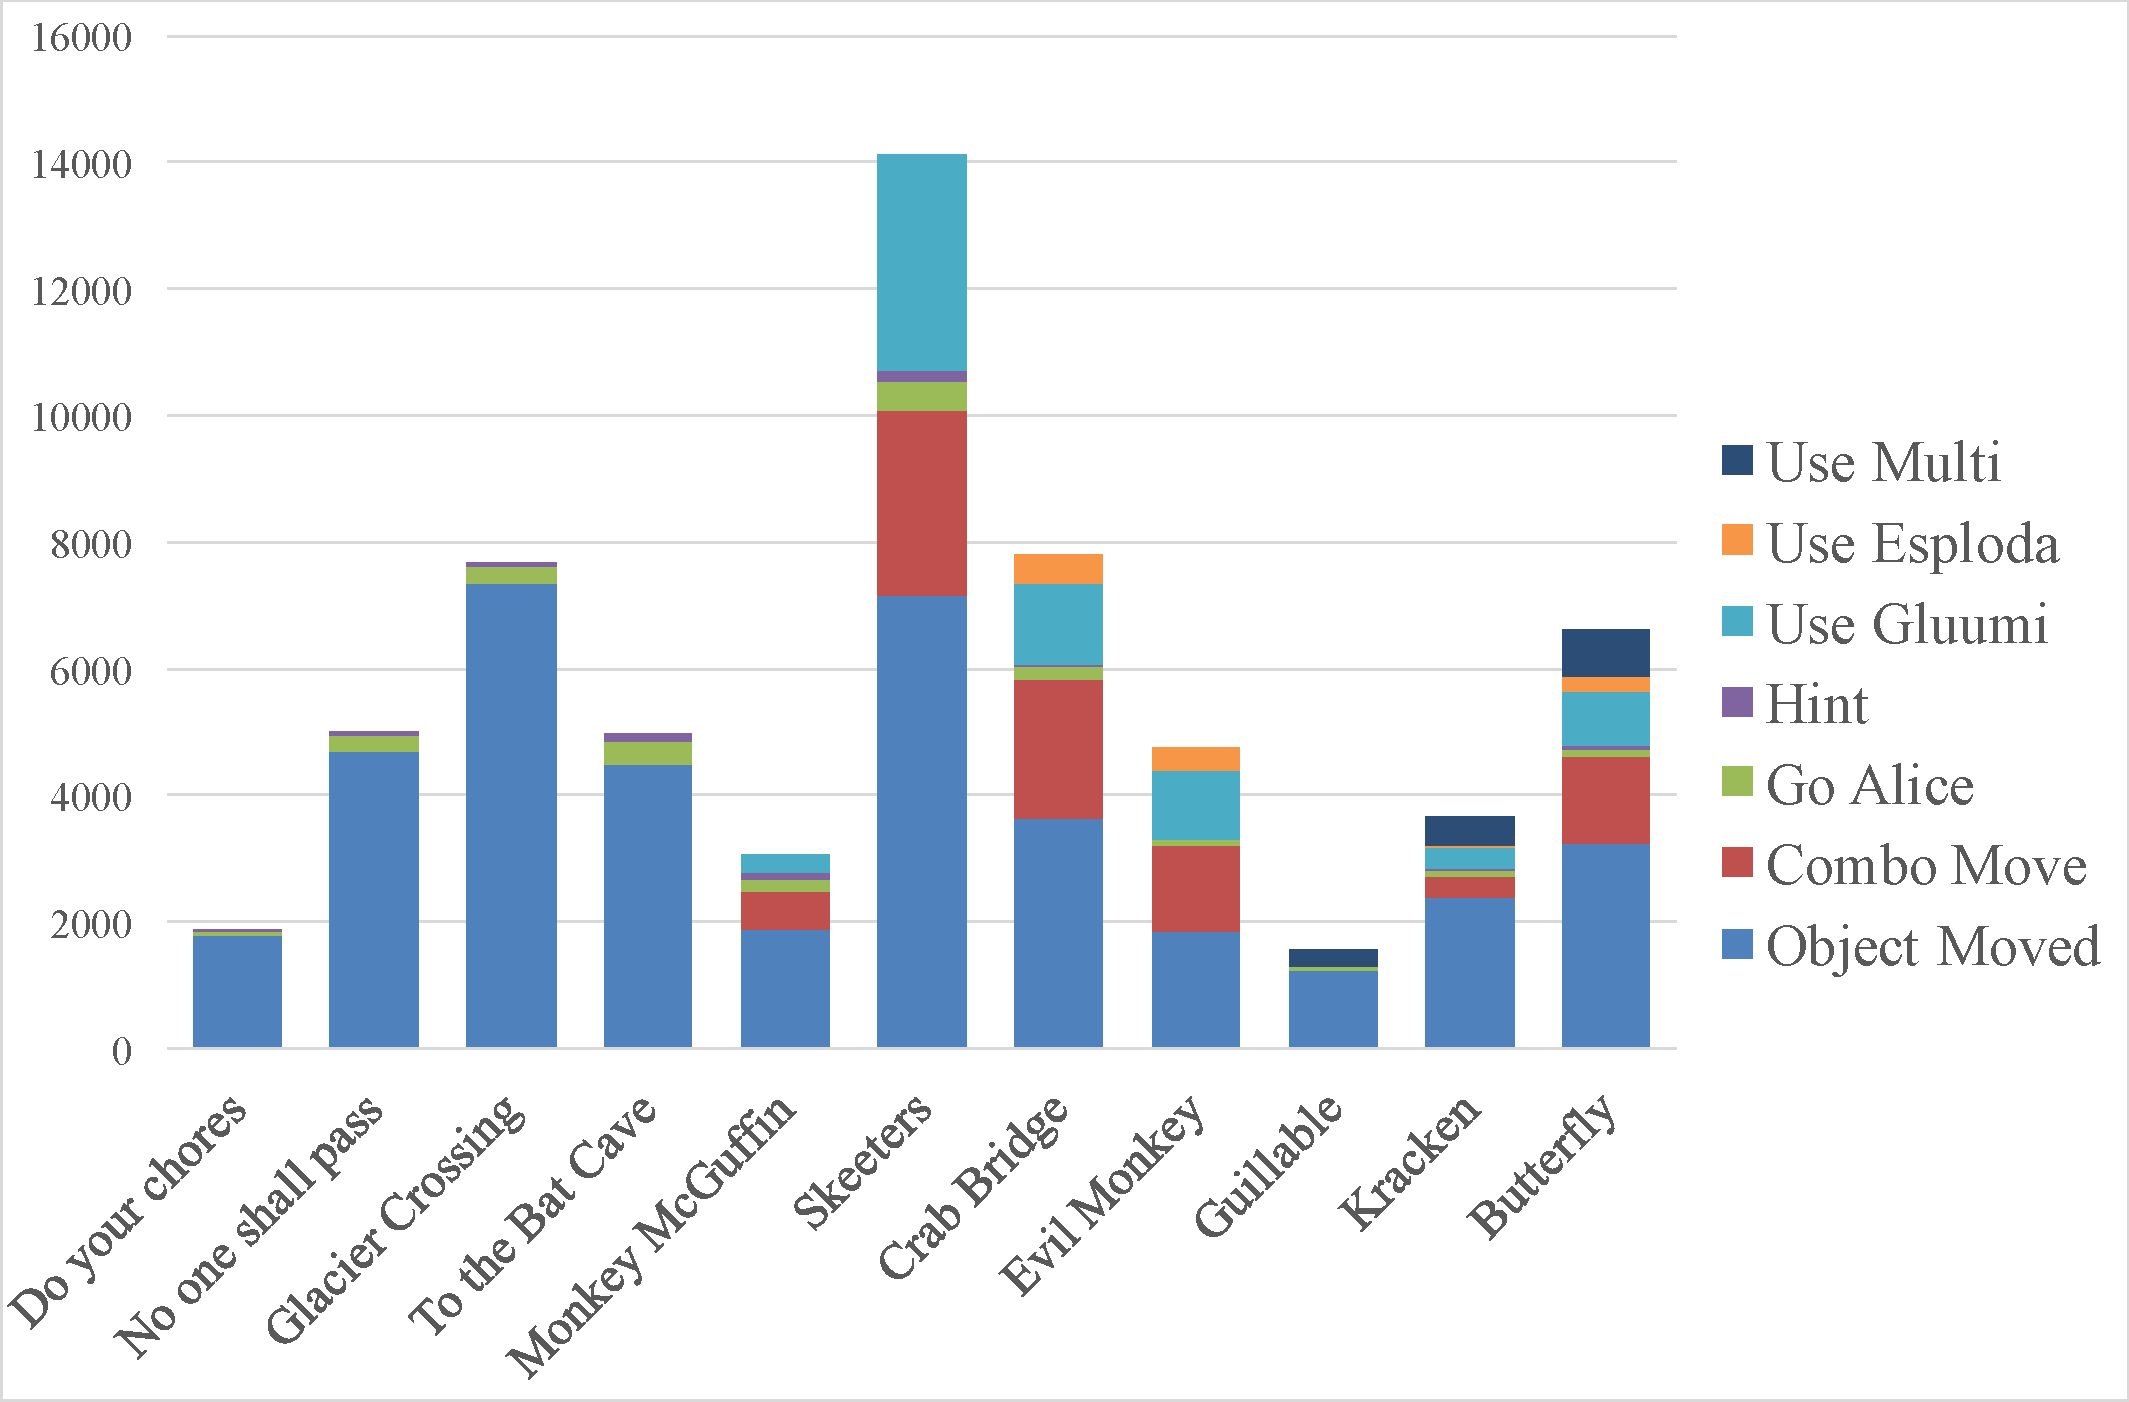
\includegraphics[width=0.9\columnwidth]{figures/frequency.pdf}
		\caption{Frequency of Events in Each Game Level}~\label{fig:frequency}
	\end{figure}	
	

	We only used the interactions of the students who participated in the post-test (77 students) in our data analysis pipeline.
	Our dataset includes the records of multiple attempts (sequence of actions) students made to solve each game level.
	Students may struggle with a game level on first attempt and change their answers multiple times to find the solution.	
	Different attempts are a rich data source for studying students' change of performance over time.	
	However, we decided to  only incorporate the first attempt in each game level in our analysis because \algname only accepts one sequence of action per game level for each student.
	Figure \ref{fig:boxplot} shows the boxplot of sequence length in each game level. 
	\newline
	\newline
	

	\begin{figure}
		\centering
		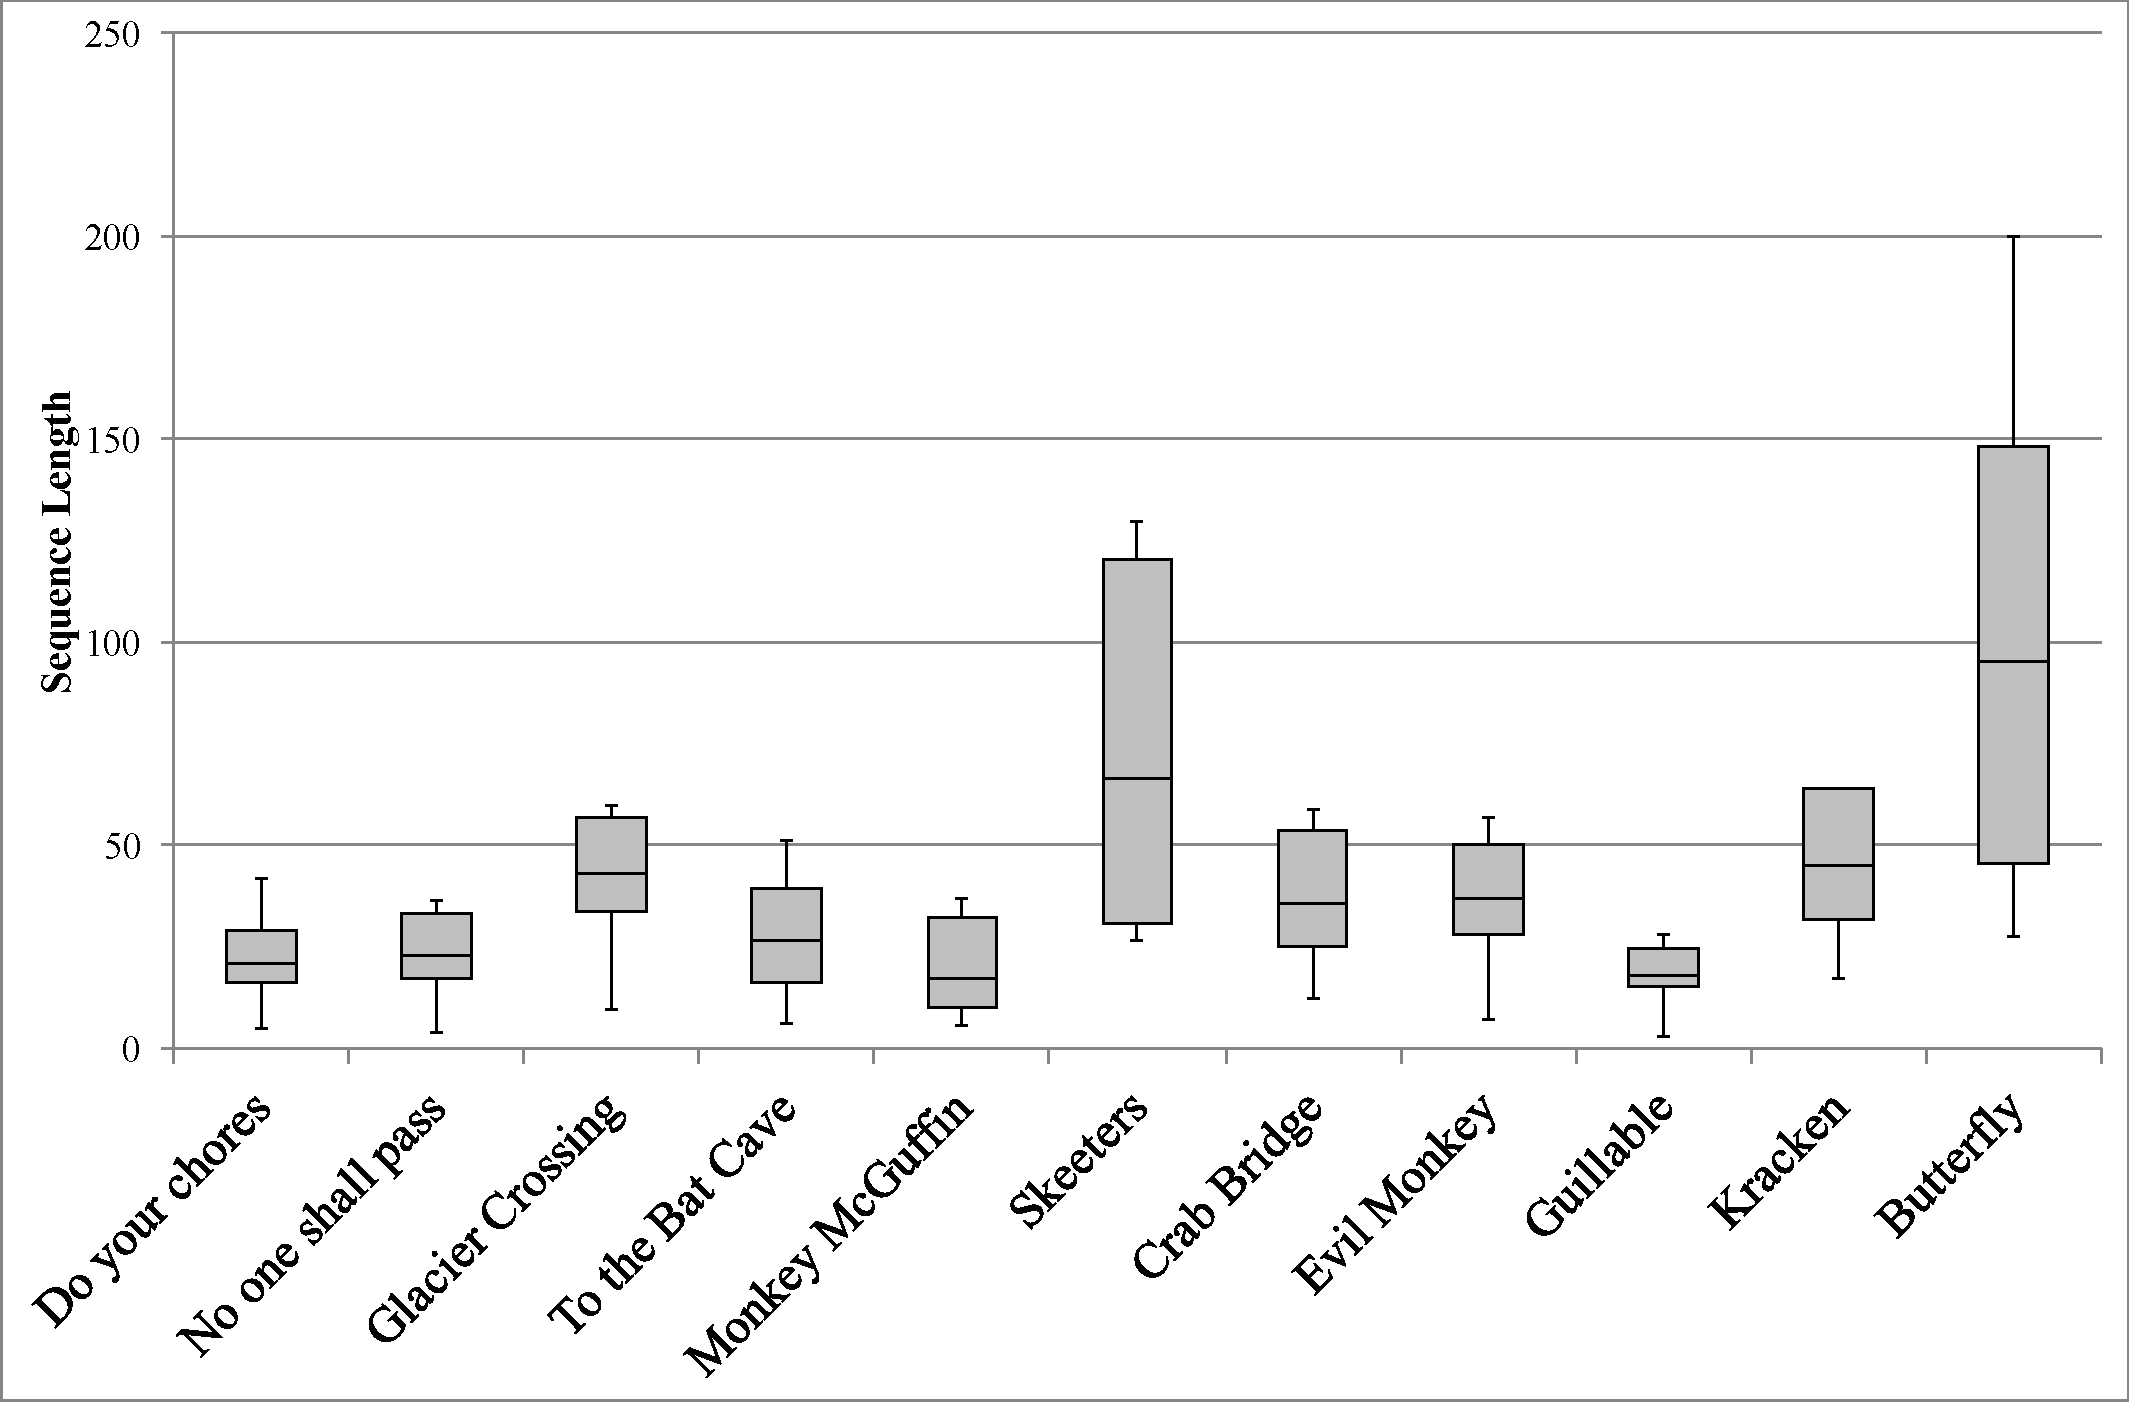
\includegraphics[width=0.9\columnwidth]{figures/boxplot.pdf}
		\caption{Boxplot of Sequence Length in Each Game Level}~\label{fig:boxplot}
	\end{figure}
		

	\subsection{Experimental Setup}
	We divide students into two groups, one (80\%) for training and development purposes, and the other (20\%) for test and verification.
	In the discretization phase, we transformed the log data from slot-and-filler structures for each game level into sequences of multinomial variables that can be used as evidence for learning for each student.
	In the sequence modeling phase, we use the multinomial sequences of students in the development set (80\%) to train two HMMs that that represent high- and low-performing students.
	In the regression phase, we use the likelihood of students' sequences in order to build a regression model that is predictive of the post-test results.
	Finally, we test the regression model on the held-out set (20\%) and report the results.
	
	\subsection{Results}
	
	
	We evaluate two implementations of SPRING, each of them using two ($K=2$) HMMs for each game level as described previously--- one for high-performing students and one for low-performing students:
	\begin{itemize}
		\item \algname ($H=1$)  uses an HMM with only one hidden state. 
		It is a model with no memory (no temporal information), because  it only consider the distribution of different observations in a sequence (as a Gaussian Mixture Model).
		This model evaluates the effect of our discretization step because it only considers the distribution of descretized observations in a sequence to distinguish between high- and low-performing students.
				
		
		\item \algname ($H^*$) learns the best number of states for each game level based on the training examples using a Hierarchical Dirichlet Prior~\cite{fox2008hdp}.
	\end{itemize} 
	
	Additionally, we evaluate two baseline methods:
	\begin{itemize}
		\item Success / Failure: A regression model with eleven binary features. Each feature represents whether a student  successfully passed each of the 11 different mini-games on the first attempt.
		\item Sequence Length: A regression model that uses the normalized sequence lengths in each game level. 
	\end{itemize}
	
	
	Table \ref{tab:results} summarizes our results.
	We use each method to predict the students the assessment score of the students in the test set.
	We compare the predictions to true scores using popular evaluation metrics:
	Pearson product-moment correlation coefficient ($R$), Spearman rank correlation $\rho$, mean absolute error (MAE) and root mean squared error (RMSE). 
	The best performing model according to all of the metrics is \algname~$H^*$. 
	
	
	\begin{table}[tbh]
		\centering
		\begin{tabular}{@{}lllll@{}}
			\toprule
			\begin{tabular}[c]{@{}l@{}}\textbf{Predictive Features}\end{tabular}            & \begin{tabular}[c]{@{}l@{}}\textbf{$R$}\end{tabular} & \begin{tabular}[c]{@{}l@{}}\textbf{$\rho$}\end{tabular} & \begin{tabular}[c]{@{}l@{}}\textbf{MAE}\end{tabular} & \textbf{RMSE}\\ \midrule
			\begin{tabular}[c]{@{}l@{}}Sequence Length (Normal)\end{tabular} & 0.15                                                     & 0.35                                                 & 2.93                                                          & 3.61 \\
			Success / Failure                                                      & 0.02                                                     & 0.16                                                 & 3.21                                                          & 4.08 \\
			\algname ($K=2, H=1$)                                                                                                        & 0.17                                                 &   0.25                                                        &
			3.60 & 3.10 \\ 
			\textbf{\algname ($K=2, H^*$)}                                                      & \textbf{0.55}                                                     & \textbf{0.51}                                                 & \textbf{2.84}                                                          & \textbf{3.35} \\ \bottomrule
		\end{tabular}
		\caption{The results of predicting post-test scores using three different feature sets.}~\label{tab:results}	
	\end{table}
	
	
	The baselines and \algname have positive correlation with the true values.
	However, the correlation is statistically significant only for \algname $H^*$ (one-sided $t$-test: $r=0.55$, $n=15$, and $p < 0.05$).
	This suggests that the predicted scores of \algname $H^*$ are positively correlated with the true assessment scores.
	
	We also calculated the absolute difference between the true and predicted post-test scores for all of the students based on each model.
	We used a paired one-sided $t$-test (n=15) to judge the significance of improvement over the baselines.
	We cannot reject the null hypothesis that the baselines are as good, or better than  \algname ($p=0.20$ over the Success/Failure baseline and $p=0.26$ over the Sequence Length baseline).
	Our results suggests that eventhough there is a positive correlation between the true and \algname's predicted post-test scores, the improvement in terms of MAE is not conclusive. 
	This effect is clearly observable in Table \ref{tab:results} where a 0.4 improvement in correlation over the first baseline resulted in 0.09 and 0.26 improvement over MAE and RMSE respectively. 
	
	The Pearson correlation coefficient and the MAE disagree in terms of  statistical significance.
	It is unclear which evaluation metric is better for our application.
	Future research could investigate how to evaluate invisible assessment systems, as well as replicate our results with larger datasets to see if the observed trend continues.
	A possible explanation of why the MAE is not significant is that our dataset is too small.
	Our held-out set contains only 15 students and a few of them achieved poor performance results in the post-test while successfully finishing most of the game levels.
	A  limitation of our approach is that our student performance clustering phase uses the post-test scores (independent variable) to divide students into high- and low-performance groups. 
	In order to avoid using information from the independent variable to calculate the features of our regression model, we are using an 80\%-20\% split to validate the results instead of for example using a 10-fold cross validation.
	This design decision, while necessary, reduces the sample size further.
	
	
	

	
	Figure~\ref{fig:regression} compares the true values against the predicted values, the regression line was calculated  using LASSO and the 95\% confidence interval is plotted.
	The regression model  provides us with an insight into how important each game level is in distinguishing between high- and low-performing students. 
	Table \ref{tab:regrweights} shows the weights of each game level in the best performing model.
	As it is shown in the table, game level 11 (\textit{You Kraken Me Up!} -- screenshot Figure~\ref{fig:figurekracken}), has the highest weight in the regression model. 
	This tells us that the difference between the sequence of student interactions in this game level has the highest factor in distinguishing between high- and low-performing students.
	The difference in predictive performance between game levels is likely related to game design. 
	Some game-levels are designed to introduce game tools and techniques while others are created to present choices to players aligned with math proficiency.
	We believe the source of difference is mainly due to the fact that finding the solution to later game levels requires mastery in all three major subskills targeted by the game design.

	
	\begin{table}[b]
		\centering
		\begin{tabular}{ll}
			\hline
			\textbf{Game Level} & \textbf{Weight} \\ \hline
			You Kraken Me Up!   & 1.686                               \\
			Skeeterz            & 1.059                               \\
			Evil Monkeys        & 1.053                               \\
			To the Bat Cave     & 0.855                               \\
			None Shall Pass     & 0.417                               \\
			...                 &                                    
		\end{tabular}
		\caption{Weights of each game level in the best performing model.}
		\label{tab:regrweights}	
	\end{table}
	
	
	\begin{figure}
		\centering
		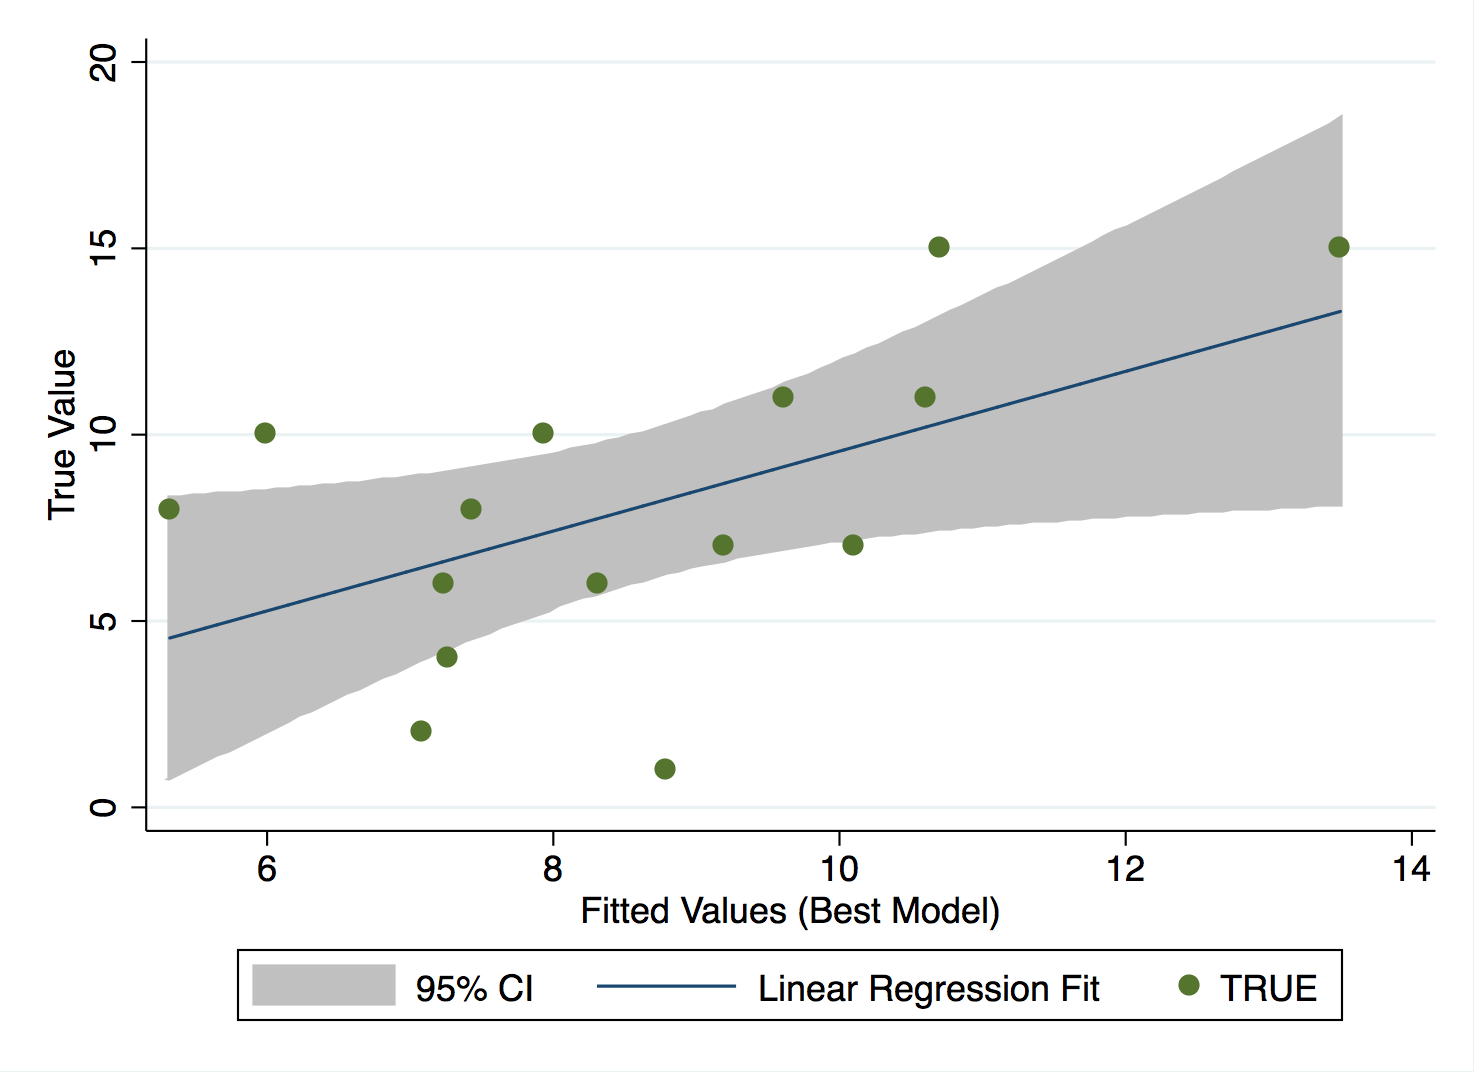
\includegraphics[width=0.9\columnwidth]{figures/regression.png}
		\caption{Results of predicting the post-test scores of the held-out set along with the regression line and 95\% interval.}~\label{fig:regression}
	\end{figure}
	
	
	\begin{figure*}
		\centering
		\begin{subfigure}[b]{.48\textwidth}
			\centering
			\resizebox{1\textwidth}{!}{
				
				\begin{tikzpicture}[->,>=stealth',shorten >=0pt,auto,node distance=.3cm,main node/.style={draw, ellipse}]
				\node[main node] (1) {S0};
				
				\node[main node] (3) [right=of 1, xshift=2cm, yshift=1cm]{S1};
				\node[main node] (2) [below=of 3, yshift=-1.3cm, xshift=.5cm, fill=lightgray]{\texttt{UseEsploda}};
				
				\node[main node] (5) [right=of 3, xshift=3.5cm, yshift=-.5cm, fill=lightgray]{\texttt{MoveCombo\_0}};
				\node[main node] (4) [above=of 5, yshift=1.5cm]{S2};
				\node[main node] (6) [below=of 5, fill=lightgray]{\texttt{UseGluumi}};
				\node[main node] (7) [below=of 6, fill=lightgray]{\texttt{MoveObject\_0}};
				
				\node[main node] (10) [right=of 4, fill=lightgray, xshift=3cm]{\texttt{MoveCombo\_4}};
				\node[main node] (9) [above=of 10, fill=lightgray]{\texttt{MoveCombo\_2}};
				\node[main node] (8) [above=of 9, fill=lightgray]{\texttt{MoveCombo\_1}};
				\node[main node] (11) [below=of 10, fill=lightgray]{\texttt{MoveCombo\_5}};
				\node[main node] (12) [below=of 11, fill=lightgray]{\texttt{Failure}};
				\node[main node] (13) [below=of 12, fill=lightgray]{\texttt{Success}};
				
				\path[thick]
				(1) edge [loop above] node [auto] {0.70} (1)
				
				(1) edge [out=-70,in=180] node [auto] {0.95} (2)
				(1) edge [out=40,in=180] node [auto] {0.28} (3)
				(3) edge [loop above] node [auto] {0.81} (3)
				
				(3) edge [out=-5,in=180] node [auto] {0.34} (5)
				(3) edge [out=-20,in=180] node [auto] {0.30} (6)
				(3) edge [out=-45,in=180] node [auto] {0.29} (7)
				(4) edge [loop above] node [auto] {0.66} (4)
				(3) edge [out=45,in=180] node [auto] {0.11} (4)
				(4) edge [out=220,in=10] node [auto] {0.29} (3)
				
				(4) edge [out=45,in=180] node [auto] {0.12} (8)
				(4) edge [out=20,in=180] node [auto] {0.12} (9)
				(4) edge [out=10,in=180] node [auto] {0.08} (10)
				(4) edge [out=0,in=180] node [auto] {0.10} (11)
				(4) edge [out=-20,in=180] node [auto] {0.19} (12)
				(4) edge [out=-45,in=180] node [auto] {0.32} (13);
				
				
				\end{tikzpicture}
			}
			
			\caption{High Performing}~\label{fig:highhmm}
		\end{subfigure}\quad
		\begin{subfigure}[b]{.48\textwidth}
			\centering
			\resizebox{1\textwidth}{!}{
				\begin{tikzpicture}[->,>=stealth',shorten >=0pt,auto,node distance=.3cm,main node/.style={draw, ellipse}]
				\node[main node] (1) {S0};
				
				\node[main node] (3) [right=of 1, xshift=2cm, yshift=1cm]{S1};
				\node[main node] (2) [below=of 3, yshift=-1.3cm, xshift=.5cm, fill=lightgray]{\texttt{UseEsploda}};
				\node[main node] (13) [below=of 2, fill=lightgray]{\texttt{MoveObject\_0}};
				
				\node[main node] (5) [right=of 3, xshift=3.5cm, yshift=-.5cm, fill=lightgray]{\texttt{MoveCombo\_0}};
				\node[main node] (4) [above=of 5, yshift=1.5cm]{S2};
				\node[main node] (6) [below=of 5, fill=lightgray]{\texttt{MoveCombo\_5}};
				\node[main node] (7) [below=of 6, fill=lightgray]{\texttt{UseGluumi}};
				
				\node[main node] (10) [right=of 4, fill=lightgray, xshift=3cm]{\texttt{MoveCombo\_4}};
				\node[main node] (9) [above=of 10, fill=lightgray]{\texttt{MoveCombo\_3}};
				\node[main node] (8) [above=of 9, fill=lightgray]{\texttt{MoveCombo\_2}};
				\node[main node] (11) [below=of 10, fill=lightgray]{\texttt{Failure}};
				\node[main node] (12) [below=of 11, fill=lightgray]{\texttt{Success}};
				
				\path[thick]
				(1) edge [loop above] node [auto] {0.76} (1)
				
				(1) edge [out=-60,in=180] node [auto] {0.43} (2)
				(1) edge [out=40,in=180] node [auto] {0.22} (3)
				(1) edge [out=-85,in=180] node [auto] {0.55} (13)
				(3) edge [out=220,in=10] node [auto] {0.12} (1)
				
				(3) edge [loop above] node [auto] {0.78} (3)
				
				(3) edge [out=-5,in=180] node [auto] {0.55} (5)
				(3) edge [out=-20,in=180] node [auto] {0.06} (6)
				(3) edge [out=-45,in=180] node [auto] {0.31} (7)
				(4) edge [loop above] node [auto] {0.71} (4)
				(3) edge [out=45,in=180] node [auto] {0.08} (4)
				(4) edge [out=220,in=10] node [auto] {0.20} (3)
				
				(4) edge [out=45,in=180] node [auto] {0.19} (8)
				(4) edge [out=20,in=180] node [auto] {0.10} (9)
				(4) edge [out=10,in=180] node [auto] {0.14} (10)
				(4) edge [out=0,in=180] node [auto] {0.19} (11)
				(4) edge [out=-20,in=180] node [auto] {0.33} (12);
				
				\end{tikzpicture}
			}\\
			\caption{Low Performing}~\label{fig:lowhmm}
		\end{subfigure}
		\caption{Learned Transition Models for One of the Game Levels}~\label{fig:highvslow}
	\end{figure*}
	

	
	Predicting post-test scores was not the only reason for designing the pipeline.
	We  also seek for a descriptive model that can give us insight into low-level patterns in student movements. 
	%This was the main idea behind using HDP-HMMs in the sequence modeling phase and our hypothesis that high-performing and low-performing students have different sequential patterns. 
	Figure~\ref{fig:highvslow} shows the difference between two HMMs learned for one of the game levels.
	In this game level in the initial state, students are presented with composite objects and they have to use the \texttt{Esploda} tool to convert them into single unit objects. 
	Then, they have to use the \texttt{Gluumi} tools to convert the single unit objects into composite objects that fit the designated area. 
	And finally, they have to move the composite object they have created into the designated area.
	For comparison purposes, we are showing a three state HMM for both high- and low-performing students and removed the edges that had probability below 0.05. 
	Figure~\ref{fig:highhmm} represents the HMM for high-performing students. 
	The three latent states, $S_{0-2}$ can be interpreted as sequential steps that students took for solving this problem. As illustrated in Figure~\ref{fig:highhmm}, high-performing students follow the expected path of using the \texttt{Esploda} tool in $S_0$, using the \texttt{Gluumi} tool in $S_1$, and then moving the composite objects into the designated areas \texttt{MoveCombo\_{ClusterID}} until they successfully finish the game.
	On the other hand, low-performing students (Figure~\ref{fig:lowhmm}) do not necessarily follow the expected path and the probability of moving object into the outlier clusters (\texttt{MoveObject\_0 and MoveCombo\_0}) is also higher across states for low-performing students.
	
	\section{Relation to Prior Work}
	\label{sec:priorwork}
	The potential of computer games for educational purposes has been of interest since nearly the beginning of video games. 
	Unlike video games, which focus on creating an entertaining experience for the user, educational games require principles and strategies that engage students while maximizing their learning gain. 
	However, games have produced mixed learning outcomes in the classroom \cite{harpstead2013search,mayo2009video} and studying student interactions is a crucial step toward understanding their learning process and improving the game environment in the future.
	
	There have been numerous attempts among the educational research community to develop analytic methods and build predictive models based on the data from educational games. 
	For example, \textit {Rumble Blocks} \cite{christel2012rumbleblocks} is a physics educational game designed to teach basic concepts of structural stability and balance to children in grades K-3 (ages 5-8 years old). 
	Harpstead et al.~\cite{harpstead2013investigating} learned a two-dimensional context-free grammar (CFG) from student interactions within the game and used a modified version of CYK algorithm to parse and extract conceptual features from student solutions.
	They used the features and performed cluster analysis of student solutions to measure how many follow the designers' envisioned path. 
	While the CFG framework offer a promising method to learn features from game activity logs, we are particularly interested in a model that can represent sequence of interactions and not the characteristics of final submission. 
	
	\textit{Crystal Island} \cite{rowe2010integrating} is an educational 3D game environment for learning microbiology in middle school. 
	Rowe and Lester \cite{rowe2010modeling} used a hand-authored dynamic Bayesian network (DBN) to model student knowledge in four broad components: narrative, content, strategy, and solution knowledge. 
	They hand picked a set of observable actions that can serve as evidence of the student's underlying knowledge in each category and defined the parameters of the model in terms of conditional probability tables for each of the network nodes (observable and latent).
	They used observations from 116 eighth-graders interacting with the game environment in 50 minute sessions.
	In order to evaluate the model, they experimented with different threshold levels to discriminate between mastered and un-mastered knowledge components and used the final estimate of student knowledge in each category (mastered vs. un-mastered) to predict their post-test results.
	The DBN framework is an example of extensive domain authoring that we are trying to avoid by using data-driven methods.
	
	One way to avoid extensive domain authoring is to use the state-action graph of the game environment. 
	States are different configurations of the game environment and actions represent different ways students can interact with the game in each state. For example, \textit {Refraction} \cite{andersen2010gameplay} is another educational game for learning about fractions by splitting laser beams into fractional amounts to target spaceships and avoid asteroids. 
	Liu et al.~\cite{liu2013predicting} created an ensemble algorithm that combines elements of Markov models, player heuristic search, and collaborative filtering techniques with state-space clustering in order to predict player movements on the last game level based on the history of movements in previous game levels. 
	Lee et al. \cite{lee2014learning} extended the former framework by building a state-action graph and using feature selection techniques to reduce the number of features for each state. 
	To ensure extensibility, they also tested the framework on another game, \textit {DragonBox}, and reported improvement over \cite{liu2013predicting}.
	While the state-action graph of the game environment offers a potential for micro-level analysis of student interactions, we are particularly interested in patterns that are representative of student proficiency.
	
	\textit {Quantum Spectre} is a more complex puzzle-style educational game designed for high school students to learn about optics. 
	Eagle et al. \cite{eagle2015measuring} used interaction networks (IN) to visualize and derive insight into students' problem solving behavior and common misconceptions. 
	They used data from 195 students in 15 classes and created the full IN of every state and possible actions for each game level. 
	Next, they used clustering to reduce the state-action space into a high level visualization of how students progress through the puzzle and classify each student interaction into four categories: correct, placement error, rotation error, and puzzle error. 
	Finally, they picked a smaller set of students (n=10) and used a linear regression model to predict their post-test results.
	The results show a direct negative relationship between science-related game play errors and the post-test scores.
	Constructing the full interaction network for each game level 
	can easily become intractable for complex games such as \textit{Alice in AreaLand}. Moreover, integrating results from multiple game levels is not straight forward since each game level has its own state-action graph and further engineering is required to extract features that are generalizable across game levels. 
	
	\section{Conclusions and Future Work}
	\label{sec:conclusion} 
	
	Educational games are an interesting source of data that provide evidence of complex cognitive behavior.
	In this study we propose a novel  data-driven method, \algname,  for student modeling in educational games. 	
	Modeling student behavior in open-ended environments such as educational games is a promising direction with applications for game designers, educators and even policy makers.
	
	
	We evaluate our models quantitatively in terms of how well we can forecast student assessments.
	%However, the discretization process, along with the use of HDP-HMMs, makes 
	We suggest that the models learned can be interpreted and can provide insight into how students  learn.
	Additionally,  the parameters of the regression model quantify how much an educational game is useful in distinguishing between high- and low-performing students.

	%fTo demonstrate the effectiveness of our framework, we use features from it to predict the post-test results using a regression model and suggested improvement over two  baselines.
	
	%In this paper, we present a data analysis framework that is able to learn a model from game activity logs that is predictive of student proficiency with minimum reliance on expert knowledge about the game environment. 
	%One of the key drawbacks of model-free methods is that their results are difficult to interpret. 
	
	There are many possible directions for future work. 
	On a lower level we can integrate the discretization and sequence modeling step by employing Hidden Markov Models that accepts slot and filler sequences as input.
	On a higher level, instead of dividing students into two groups (high- and low-performing), we can use the HMM to cluster students \cite{bicego2003similarity,smyth1997clustering} into more groups that might be  more representative of different approaches students follow to solve each game level. 
	We can also replace our regression model with a more powerful ensemble method that considers different subskills in order to integrate features of each game level to predict the post-test scores.
	
	Even though we only evaluated \algname using data from a single game, the algorithm  may be useful for  similar gaming environments that use slot-and-filler structures to log student interactions with the system. 
	 We are optimistic that our approach may be useful to make assessment less intrusive and better embedded to classroom education.
	%able to build a model that detects incorrect strategies or common misconceptions that can be used in a dynamic hinting system to increase player engagement and learning.
	
	\bibliographystyle{SIGCHI-Reference-Format}
	\balance
	\bibliography{references}
	
\end{document}